\documentclass[aspectratio=169,10pt]{beamer}

% -------------------------------------------------------
% KAUST Academy Template  --  Python Pathway · Course 1
% -------------------------------------------------------

\usepackage[T1]{fontenc}
\usepackage[utf8]{inputenc}
\usepackage{tikz}
\usetikzlibrary{arrows.meta,positioning,shadows.blur,calc,fit,
                decorations.pathreplacing,shapes.geometric}
\usepackage{array}
\usepackage{tabularx}
\usepackage{booktabs}
\usepackage[most]{tcolorbox}
\usepackage{ragged2e}
\usepackage{adjustbox}
\usepackage{xcolor}
\usepackage{listings}
\usepackage{graphicx}
\usepackage{subcaption}
\usepackage{amsmath,amssymb}
\usepackage{multirow}
\usepackage{multicol}
\usepackage{hyperref}
\hypersetup{colorlinks=true}

% -------------------------------------------------------
% KAUST Stanford Beamer Theme
% (beamerthemeStanford.sty, beamercolorthemestanford.sty,
%  beamerouterthemesimplefooter.sty must be on the TeX path
%  or in the same directory as this file)
% -------------------------------------------------------
\usetheme{Stanford}

\logo{%
  
\includegraphics[height=0.3in]{style_files/kaust_academy_logo.png}\hspace{0.06in}%
  
\includegraphics[height=0.3in]{style_files/LMHLogo_crest.png}%
}

\makeatletter
\let\@@magyar@captionfix\relax
\makeatother

\setbeamertemplate{itemize items}[default]
\setbeamertemplate{itemize subitem}[circle]
\setbeamertemplate{caption}[numbered]
\setbeamertemplate{navigation symbols}{}

% -------------------------------------------------------
% Color Palette  (PrimaryBlue = KAUST Blue RGB 0,51,102)
% -------------------------------------------------------
\definecolor{PrimaryBlue}{RGB}{0,51,102}
\definecolor{LightGray}{RGB}{245,247,250}
\definecolor{LineGray}{RGB}{180,180,180}
\definecolor{CodeGreen}{RGB}{0,118,83}
\definecolor{CodeRed}{RGB}{190,30,30}
\definecolor{CodeBlue}{RGB}{0,55,130}
\definecolor{CodePurple}{RGB}{114,47,145}

% -------------------------------------------------------
% Custom Commands
% -------------------------------------------------------
\newcommand{\blueball}{%
  \tikz[baseline=-0.6ex]\shade[ball color=PrimaryBlue] (0,0) circle (0.065cm);%
}
\setbeamertemplate{itemize item}{\blueball}
\setbeamertemplate{itemize subitem}{\blueball}
\setlength{\leftmargini}{1.1cm}
\setlength{\leftmarginii}{0.8cm}

\newcommand{\keyword}[1]{\textcolor{PrimaryBlue}{\textbf{#1}}}
\newcommand{\myitem}[1]{\item #1\vspace{0.04cm}}

% Numbered-circle helper
\newcommand{\numcircle}[1]{%
  \tikz[baseline=-0.7ex]\node[circle,shade,ball color=PrimaryBlue,
    text=white,font=\scriptsize\bfseries,inner sep=1.2pt,
    minimum size=0.18cm]{#1};%
}
\newenvironment{numberedlines}%
  {\begin{tabular}{@{}p{0.42cm}p{\dimexpr\textwidth-0.75cm\relax}@{}}}%
  {\end{tabular}}
\newcommand{\nline}[2]{\numcircle{#1} & #2 \\[0.13cm]}

% Placeholder badge (for notebook-covered slides)
\newcommand{\placeholderbadge}{%
  \begin{tikzpicture}[remember picture,overlay]
    \node[anchor=north east,fill=orange!18,draw=orange!70!black,
          rounded corners=1mm,inner xsep=2mm,inner ysep=0.8mm,
          font=\scriptsize\bfseries,text=orange!55!black]
      at ([xshift=-0.28cm,yshift=-1.0cm]current page.north east)
      {PLACEHOLDER --- notebook will cover this};
  \end{tikzpicture}%
}

% -------------------------------------------------------
% tcolorbox Styles
% -------------------------------------------------------
\tcbset{
  lecturebox/.style={
    enhanced,
    colback=LightGray,
    colframe=LineGray,
    boxrule=0.35pt,
    arc=2mm,
    left=1.6mm,right=1.6mm,top=0.8mm,bottom=0.8mm,
    drop shadow={black!45!white,opacity=0.35,
                 shadow xshift=1.2mm,shadow yshift=-1.2mm},
    fonttitle=\normalsize,
    coltitle=white,
    colbacktitle=PrimaryBlue,
    boxed title style={arc=2mm,boxrule=0pt},
    attach boxed title to top left={xshift=0mm,yshift=-0.5mm},
    boxed title size=title,
  },
  plainbox/.style={
    enhanced,
    colback=LightGray,
    colframe=LineGray,
    boxrule=0.35pt,
    arc=2mm,
    left=1.6mm,right=1.6mm,top=0.8mm,bottom=0.8mm,
  }
}

% -------------------------------------------------------
% Python / Code Listing Styles
% -------------------------------------------------------
\lstdefinestyle{pycode}{
  language=Python,
  basicstyle=\ttfamily\scriptsize,
  columns=fullflexible,keepspaces=true,showstringspaces=false,
  breaklines=true,frame=single,rulecolor=\color{LineGray},
  backgroundcolor=\color{gray!6},
  keywordstyle=\color{CodeBlue}\bfseries,
  stringstyle=\color{CodeRed},
  commentstyle=\color{CodeGreen},
  xleftmargin=0pt,xrightmargin=0pt
}
\lstdefinestyle{pycodesmall}{style=pycode,basicstyle=\ttfamily\tiny}
\lstdefinestyle{pycodelarge}{language=Python,
  basicstyle=\ttfamily\large,columns=fullflexible,
  keepspaces=true,showstringspaces=false,frame=single,
  rulecolor=\color{LineGray},backgroundcolor=\color{gray!6},
  keywordstyle=\color{CodeBlue}\bfseries,
  stringstyle=\color{CodeRed},commentstyle=\color{CodeGreen},
  xleftmargin=0pt,xrightmargin=0pt}
\lstdefinestyle{pycodemedium}{language=Python,
  basicstyle=\ttfamily\normalsize,columns=fullflexible,
  keepspaces=true,showstringspaces=false,frame=single,
  rulecolor=\color{LineGray},backgroundcolor=\color{gray!6},
  keywordstyle=\color{CodeBlue}\bfseries,
  stringstyle=\color{CodeRed},commentstyle=\color{CodeGreen},
  xleftmargin=0pt,xrightmargin=0pt}
\lstdefinestyle{termcode}{basicstyle=\ttfamily\large,
  columns=fullflexible,keepspaces=true,showstringspaces=false,
  frame=single,rulecolor=\color{LineGray},backgroundcolor=\color{gray!6}}
\lstdefinestyle{outcode}{basicstyle=\ttfamily\large,
  columns=fullflexible,keepspaces=true,showstringspaces=false,
  frame=single,rulecolor=\color{LineGray},backgroundcolor=\color{gray!6}}
\lstdefinestyle{pseudo}{basicstyle=\ttfamily\large,
  columns=fullflexible,keepspaces=true,showstringspaces=false,
  frame=single,rulecolor=\color{LineGray},backgroundcolor=\color{gray!6},
  xleftmargin=0pt,xrightmargin=0pt}
\lstdefinestyle{pseudocode}{basicstyle=\ttfamily\large,
  columns=fullflexible,keepspaces=true,showstringspaces=false,
  frame=single,rulecolor=\color{LineGray},backgroundcolor=\color{gray!6}}

% -------------------------------------------------------
% TikZ Diagram Styles
% -------------------------------------------------------
\tikzset{
  flowbox/.style={draw=black!85,rounded corners=2mm,fill=LightGray,
    minimum width=2.15cm,minimum height=0.68cm,align=center,font=\normalsize},
  flowarrow/.style={-{Latex[length=2.5mm,width=2.0mm]},
    line width=0.8pt,draw=PrimaryBlue},
  levelbox/.style={draw=black!70,rounded corners=2mm,fill=LightGray,
    text width=3.65cm,minimum height=1.15cm,align=center,font=\normalsize},
  codebox/.style={draw=black!70,rounded corners=2mm,fill=gray!7,
    text width=3.3cm,minimum height=1.1cm,align=center,font=\normalsize},
  terminator/.style={draw,rounded corners=2.5mm,minimum width=2.4cm,
    minimum height=0.48cm,fill=gray!5,align=center},
  process/.style={draw,rectangle,minimum width=2.3cm,
    minimum height=0.52cm,fill=gray!5,align=center},
  decision/.style={draw,diamond,aspect=2.05,inner sep=1.3pt,
    minimum width=2.75cm,minimum height=1.1cm,fill=gray!5,align=center},
  io/.style={draw,trapezium,trapezium left angle=70,
    trapezium right angle=110,minimum width=2.4cm,
    minimum height=0.55cm,fill=gray!5,align=center},
}

% -------------------------------------------------------
% Presentation Metadata
% -------------------------------------------------------
\title[Introduction to Data Science]{Introduction to Data Science}
% \subtitle{AI Specialization $\cdot$ Python Pathway}
\author[KAUST Academy]{%
  \begin{tabular}{c}
    \Large Naeemullah Khan
  \end{tabular}
  \vspace{-3ex}%
}
\institute{%
  \vskip 8pt
  \begin{figure}
    \centering
    
\includegraphics[height=0.5in]{style_files/kaust_logo.png}\qquad
    
\includegraphics[height=0.5in]{style_files/LMHLogo.png}
  \end{figure}
  \vskip 6pt
  KAUST Academy\\[3pt]
  King Abdullah University of Science and Technology\\[3pt]
  Stage~1 $\cdot$ Course~4%
}
\date{\today}

% =====================================================

% -------------------------------------------------------
% Course 4 extra commands
% -------------------------------------------------------
\newcommand{\codeword}[1]{\texttt{#1}}
\newcommand{\code}[1]{\texttt{#1}}
\newcommand{\blue}[1]{\textcolor{PrimaryBlue}{\textbf{#1}}}
\newenvironment{bluebox}[1]{%
  \vspace{0.08cm}\begin{tcolorbox}[lecturebox,title={#1},fontupper=\small]%
}{\end{tcolorbox}\vspace{0.05cm}}
\lstdefinestyle{py}{language=Python,basicstyle=\ttfamily\scriptsize,
  keywordstyle=\color{CodeBlue}\bfseries,stringstyle=\color{CodeRed},
  commentstyle=\color{CodeGreen},showstringspaces=false,
  backgroundcolor=\color{gray!6},frame=single,framerule=0.3pt,
  rulecolor=\color{LineGray},columns=fullflexible,keepspaces=true,
  breaklines=true}

\begin{document}


% ============================================================
% COURSE TITLE SLIDE
% ============================================================
% ------------------------------------------
% Title / Cover Slide
% ------------------------------------------
\begin{noheadline}
\begin{frame}
\maketitle
\end{frame}
\end{noheadline}



% ============================================================
% MODULE 1 TITLE SLIDE
% ============================================================
\begin{noheadline}
\begin{frame}
\frametitle{Module 1: NUMERICAL COMPUTING WITH NUMPY}
\vspace{1.2cm}
\begin{center}
  {\fontsize{30}{36}\selectfont\textbf{Module 1}}\\[0.35cm]
  {\fontsize{20}{26}\selectfont NUMERICAL COMPUTING WITH NUMPY}\\[0.7cm]
  \tcbox[colback=PrimaryBlue!6,colframe=PrimaryBlue,arc=3mm,boxrule=1pt,left=8mm,right=8mm,top=4mm,bottom=4mm,fontupper=\Large]{Arrays, vectorized operations, and linear algebra}
\end{center}
\end{frame}
\end{noheadline}


% ============================================================
% MODULE 1 CONTENT SLIDE
% ============================================================
\begin{frame}
\frametitle{Module Content}
\small
This module covers building and manipulating arrays efficiently for numerical and scientific computing.

\vspace{0.16cm}
\begin{columns}[T,totalwidth=0.96\textwidth]
\begin{column}{0.48\textwidth}
\begin{itemize}\setlength\itemsep{0.08cm}
  \item \keyword{Why NumPy?}: fast fixed-type arrays vs.\ Python lists.
  \item \keyword{Creating arrays}: from lists, ranges, zeros, ones, and random values.
  \item \keyword{Attributes and dtypes}: shape, size, and type system.
  \item \keyword{Indexing and slicing}: 1-D, 2-D, and N-D access patterns.
  \item \keyword{Boolean and fancy indexing}: filter and select with conditions.
\end{itemize}
\end{column}
\begin{column}{0.48\textwidth}
\begin{itemize}\setlength\itemsep{0.08cm}
  \item \keyword{Broadcasting}: element-wise operations across different shapes.
  \item \keyword{Ufuncs and aggregations}: vectorized math and reductions.
  \item \keyword{Reshaping and combining}: \codeword{reshape}, \codeword{stack}, \codeword{concatenate}.
  \item \keyword{Linear algebra and random numbers}: \codeword{np.linalg} and \codeword{np.random}.
  \item \keyword{Saving and loading}: \codeword{.npy}, \codeword{.npz}, and performance tips.
\end{itemize}
\end{column}
\end{columns}
\end{frame}


% ============================================================
% 5.1 NUMPY FUNDAMENTALS
% ============================================================
\begin{frame}[fragile]
\frametitle{Why NumPy?}
\small
Python lists are flexible but slow for numerical work. \keyword{NumPy} provides a fixed-type, fixed-size array (\codeword{ndarray}) and runs operations in optimized C code. It is the foundation of the entire scientific Python ecosystem.

\vspace{0.15cm}
\begin{lstlisting}[style=pycode]
import numpy as np
import time

# Pure Python loop
xs = list(range(1_000_000))
t0 = time.perf_counter()
ys = [x * 2 for x in xs]
print("loop:", time.perf_counter() - t0)        # ~ 0.05 s

# NumPy vectorized
arr = np.arange(1_000_000)
t0 = time.perf_counter()
arr2 = arr * 2
print("numpy:", time.perf_counter() - t0)       # ~ 0.001 s
\end{lstlisting}

\begin{tcolorbox}[lecturebox,title=Key idea]
NumPy is fast because it stores data in \keyword{contiguous memory} with a single dtype, and operates on whole arrays at once instead of element by element in Python.
\end{tcolorbox}
\end{frame}


\begin{frame}[fragile]
\frametitle{Creating Arrays}
\small
NumPy offers many ways to build arrays. Pick the constructor that best expresses your intent.

\vspace{0.12cm}
\begin{lstlisting}[style=pycode]
import numpy as np

np.array([1, 2, 3])             # from a Python list
np.zeros((3, 4))                # 3x4 array of zeros
np.ones((2, 5))                 # 2x5 array of ones
np.full((2, 2), 7)              # filled with a constant
np.eye(4)                       # 4x4 identity matrix

np.arange(0, 10, 2)             # [0, 2, 4, 6, 8]
np.linspace(0, 1, 5)            # 5 evenly spaced values: [0, 0.25, 0.5, 0.75, 1]
\end{lstlisting}

\begin{bluebox}{arange vs.\ linspace}
\codeword{arange(start, stop, step)} controls the \keyword{step}. \codeword{linspace(start, stop, n)} controls the \keyword{number of points}. Use \codeword{linspace} when you need a precise count (e.g.\ for plotting).
\end{bluebox}
\end{frame}


\begin{frame}[fragile]
\frametitle{Array Attributes and dtypes}
\small
Every \codeword{ndarray} carries metadata that describes its shape and storage.

\vspace{0.12cm}
\begin{lstlisting}[style=pycode]
a = np.array([[1, 2, 3], [4, 5, 6]], dtype=np.float32)

a.shape        # (2, 3)        -> rows, cols
a.ndim         # 2             -> number of dimensions
a.size         # 6             -> total elements
a.dtype        # float32        -> element type
a.itemsize     # 4             -> bytes per element
a.nbytes       # 24            -> total bytes
\end{lstlisting}

\renewcommand{\arraystretch}{1.20}
\begin{tabularx}{\linewidth}{>{\bfseries}p{2.4cm}X}
\toprule
dtype & When to use \\
\midrule
\code{float64} & Default for floats. Maximum precision. \\
\code{float32} & Half the memory. Standard on \keyword{GPUs} and most ML frameworks. \\
\code{int32 / int64} & Integers. \codeword{int64} default on 64-bit systems. \\
\code{bool} & 1 byte each. Used by boolean indexing. \\
\bottomrule
\end{tabularx}
\end{frame}


\begin{frame}[fragile]
\frametitle{Indexing and Slicing}
\small
NumPy uses comma-separated indexing for multi-dimensional arrays. Slicing returns a \keyword{view}, not a copy.

\vspace{0.12cm}
\begin{lstlisting}[style=pycode]
a = np.array([[1, 2, 3, 4],
              [5, 6, 7, 8],
              [9, 10, 11, 12]])

a[0, 0]            # 1            -> single element
a[1]               # [5, 6, 7, 8] -> entire row
a[:, 2]            # [3, 7, 11]   -> entire column
a[0:2, 1:3]        # [[2, 3], [6, 7]]   -> submatrix

a[1, 2] = 99       # mutates the original

# 3D arrays follow the same pattern
cube = np.zeros((4, 5, 6))     # shape (depth, rows, cols)
cube[0, :, :].shape            # (5, 6)
\end{lstlisting}

\begin{bluebox}{Slice vs.\ copy}
\codeword{a[0:2, 1:3]} is a \keyword{view} into the original. To get an independent copy, use \codeword{a[0:2, 1:3].copy()}.
\end{bluebox}
\end{frame}


\begin{frame}[fragile]
\frametitle{Boolean and Fancy Indexing}
\small
Index by a boolean mask (filter) or by a list of integer positions (gather).

\vspace{0.12cm}
\begin{lstlisting}[style=pycode]
a = np.array([10, 20, 30, 40, 50])

# Boolean indexing: filter by condition
mask = a > 25
print(mask)              # [False False  True  True  True]
print(a[mask])           # [30 40 50]
print(a[a > 25])         # same thing in one line

a[a > 25] = 0            # set matching elements

# Fancy indexing: pick by integer positions
idx = [0, 2, 4]
print(a[idx])            # [10 30 50]

# Combined conditions: use & and | (NOT and / or)
print(a[(a > 10) & (a < 50)])
\end{lstlisting}

\begin{tcolorbox}[lecturebox,title=Why this matters]
Boolean masks are the NumPy / Pandas way to filter data. They replace explicit \codeword{for} loops in almost every data-cleaning task.
\end{tcolorbox}
\end{frame}


\begin{frame}[fragile]
\frametitle{Element-wise Operations and Broadcasting}
\small
Arithmetic on arrays is \keyword{element-wise}. When shapes differ, NumPy uses \keyword{broadcasting} to align them.

\vspace{0.12cm}
\begin{lstlisting}[style=pycode]
a = np.array([1, 2, 3])
b = np.array([10, 20, 30])

a + b          # [11, 22, 33]   element-wise
a * b          # [10, 40, 90]
a ** 2         # [1, 4, 9]
a + 100        # [101, 102, 103]    scalar broadcasts

# 2D broadcasting
M = np.ones((3, 4))     # shape (3, 4)
v = np.array([1, 2, 3, 4])
print(M + v)            # v is broadcast across each row
\end{lstlisting}

\begin{tcolorbox}[lecturebox,title=Broadcasting rules]
Two shapes are compatible when, comparing dimensions \keyword{from the right}: each pair is either equal, or one of them is 1. The size-1 dimension is then \keyword{stretched} to match the other.

\vspace{0.06cm}
Example: \codeword{(3, 4)} with \codeword{(4,)} aligns as \codeword{(3, 4)} with \codeword{(1, 4)} \(\Rightarrow\) compatible.
\end{tcolorbox}
\end{frame}


\begin{frame}[fragile]
\frametitle{Universal Functions and Aggregations}
\small
\keyword{Universal functions} (ufuncs) apply element-wise. \keyword{Aggregations} reduce an array along an axis.

\vspace{0.12cm}
\begin{lstlisting}[style=pycode]
a = np.array([[1, 2, 3],
              [4, 5, 6]])

# Ufuncs (element-wise)
np.sqrt(a)
np.exp(a)
np.log(a)
np.maximum(a, 3)              # element-wise max with a scalar

# Aggregations (reduce)
a.sum()           # 21         -> across all elements
a.mean()          # 3.5
a.std()           # standard deviation
a.min(),  a.max()
a.argmin(),  a.argmax()       # index of min / max

# Axis parameter
a.sum(axis=0)     # [5, 7, 9]   -> sum down columns
a.sum(axis=1)     # [6, 15]     -> sum across rows
a.cumsum(axis=1)  # cumulative
\end{lstlisting}
\end{frame}


\begin{frame}[fragile]
\frametitle{Reshaping and Combining Arrays}
\small
\begin{lstlisting}[style=pycode]
a = np.arange(12)

a.reshape(3, 4)           # 3 rows, 4 cols
a.reshape(3, -1)          # -1 means "infer this dimension"
a.ravel()                 # flatten -> view (when possible)
a.flatten()               # flatten -> always a copy

M = np.array([[1, 2], [3, 4]])
M.T                       # transpose

# Combining
np.concatenate([a, a], axis=0)
np.stack([a, a])          # adds a NEW axis
np.vstack([M, M])         # vertical stack  -> rows
np.hstack([M, M])         # horizontal stack -> cols
np.split(a, 3)            # [array1, array2, array3]
\end{lstlisting}

\begin{bluebox}{When shapes do not match}
Most reshape errors come from forgetting \codeword{axis}, or using a tuple shape that does not multiply to the original size. Always check \codeword{a.shape} before and after.
\end{bluebox}
\end{frame}


\begin{frame}[fragile]
\frametitle{Linear Algebra and Random Numbers}
\small
NumPy ships with \codeword{np.linalg} for linear algebra and \codeword{np.random} for sampling. Both are essential in machine learning.

\vspace{0.12cm}
\begin{lstlisting}[style=pycode]
A = np.array([[1, 2], [3, 4]])
B = np.array([[5, 6], [7, 8]])

A @ B                # matrix product (preferred syntax)
np.matmul(A, B)      # same thing
np.linalg.inv(A)     # inverse
np.linalg.det(A)     # determinant
np.linalg.eig(A)     # eigenvalues and eigenvectors
np.linalg.norm(A)    # Frobenius norm

# Random sampling
rng = np.random.default_rng(seed=42)        # modern API
rng.normal(0, 1, size=(3, 4))               # standard normal
rng.uniform(0, 10, size=5)
rng.integers(0, 100, size=10)
rng.choice([1, 2, 3], size=5, replace=True)
\end{lstlisting}

\begin{tcolorbox}[lecturebox,title=Reproducibility]
Always set a \codeword{seed} when you want experiments to be reproducible. The new \codeword{default\_rng()} is preferred over the older \codeword{np.random.seed()}.
\end{tcolorbox}
\end{frame}


\begin{frame}[fragile]
\frametitle{Saving, Loading, and Performance}
\small
\begin{columns}[T,totalwidth=0.98\textwidth]
\begin{column}{0.55\textwidth}
\textbf{Persistence}
\begin{lstlisting}[style=pycodesmall]
np.save("data.npy", arr)         # binary, fast
arr = np.load("data.npy")

np.savetxt("data.csv", arr,      # human-readable
           delimiter=",")
arr = np.loadtxt("data.csv",
                 delimiter=",")
\end{lstlisting}
\end{column}
\begin{column}{0.42\textwidth}
\textbf{Performance tips}
\begin{itemize}\setlength\itemsep{0.04cm}
  \item Vectorize: replace Python loops with array operations.
  \item Pick the right \keyword{dtype}: \codeword{float32} halves memory.
  \item Memory layout: \keyword{C-order} (row major, default) vs.\ \keyword{F-order} (column major).
  \item Use \codeword{np.where}, \codeword{np.select} for branching.
\end{itemize}
\end{column}
\end{columns}

\vspace{0.15cm}
\begin{bluebox}{Mental shift}
In NumPy you describe \keyword{what} you want done to the whole array. The library figures out the fast way to do it. Writing explicit element-by-element loops almost always means a slower program.
\end{bluebox}
\end{frame}


% ============================================================
% MODULE 2 TITLE SLIDE
% ============================================================
\begin{noheadline}
\begin{frame}
\frametitle{Module 2: TABULAR DATA WITH PANDAS}
\vspace{1.2cm}
\begin{center}
  {\fontsize{30}{36}\selectfont\textbf{Module 2}}\\[0.35cm]
  {\fontsize{25}{30}\selectfont TABULAR DATA WITH PANDAS}\\[0.7cm]
  \tcbox[colback=PrimaryBlue!6,colframe=PrimaryBlue,arc=3mm,boxrule=1pt,left=8mm,right=8mm,top=4mm,bottom=4mm,fontupper=\Large]{Series, DataFrames, cleaning, grouping, and merging}
\end{center}
\end{frame}
\end{noheadline}


% ============================================================
% MODULE 2 CONTENT SLIDE
% ============================================================
\begin{frame}
\frametitle{Module Content}
\small
This module covers loading, cleaning, reshaping, and analysing structured datasets using Pandas Series and DataFrames.

\vspace{0.16cm}
\begin{columns}[T,totalwidth=0.96\textwidth]
\begin{column}{0.48\textwidth}
\begin{itemize}\setlength\itemsep{0.08cm}
  \item \keyword{Series}: labeled 1-D arrays built on NumPy.
  \item \keyword{DataFrames}: tabular data with labeled rows and columns.
  \item \keyword{Indexing}: \codeword{.loc} vs.\ \codeword{.iloc} for label and positional access.
  \item \keyword{Inspecting data}: \codeword{info()}, \codeword{describe()}, and \codeword{head()}.
  \item \keyword{Missing data}: detecting, dropping, and filling \codeword{NaN}.
\end{itemize}
\end{column}
\begin{column}{0.48\textwidth}
\begin{itemize}\setlength\itemsep{0.08cm}
  \item \keyword{Type conversion, strings, and sorting}: cleaning real-world data.
  \item \keyword{GroupBy and aggregation}: split-apply-combine patterns.
  \item \keyword{Merging and joining}: combining DataFrames like SQL joins.
  \item \keyword{Apply, map, and method chaining}: expressive transformations.
  \item \keyword{Time series and categoricals}: working with dates and ordered data.
\end{itemize}
\end{column}
\end{columns}
\end{frame}


% ============================================================
% 5.2 PANDAS FUNDAMENTALS
% ============================================================
\begin{frame}[fragile]
\frametitle{From NumPy to Pandas: the Series}
\small
A \keyword{Series} is a one-dimensional NumPy array with a labeled index. Think of it as a labeled vector.

\vspace{0.12cm}
\begin{lstlisting}[style=pycode]
import pandas as pd

s = pd.Series([10, 20, 30, 40], index=["a", "b", "c", "d"])
print(s)
# a    10
# b    20
# c    30
# d    40
# dtype: int64

s["b"]            # 20    -> label-based access
s[s > 15]         # boolean filter (just like NumPy)
s.mean()          # 25.0
\end{lstlisting}

\begin{tcolorbox}[lecturebox,title=Index alignment]
When you combine two Series, Pandas \keyword{aligns by index label}, not by position. Missing labels become \codeword{NaN}. This is the single biggest difference from a plain list.
\end{tcolorbox}
\end{frame}


\begin{frame}[fragile]
\frametitle{The DataFrame: Tabular Data}
\small
A \keyword{DataFrame} is a 2-D table where every column is a Series. Columns can have different dtypes.

\vspace{0.12cm}
\begin{lstlisting}[style=pycode]
df = pd.DataFrame({
    "name":  ["Aisha", "Omar", "Lina", "Tariq"],
    "age":   [22, 25, 23, 28],
    "score": [95.0, 88.5, 91.0, 76.5],
})

# Read from common sources
pd.read_csv("data.csv")
pd.read_json("data.json")
pd.read_excel("data.xlsx")
pd.DataFrame(np_array, columns=["x", "y", "z"])
\end{lstlisting}

\renewcommand{\arraystretch}{1.20}
\begin{tabularx}{\linewidth}{>{\bfseries}p{3.6cm}X}
\toprule
Property & Meaning \\
\midrule
\code{df.columns}  & column labels \\
\code{df.index}    & row labels \\
\code{df.shape}    & \texttt{(rows, cols)} \\
\code{df["age"]}   & a single column (returns a Series) \\
\code{df[["age","score"]]} & multiple columns (returns a DataFrame) \\
\bottomrule
\end{tabularx}
\end{frame}


\begin{frame}[fragile]
\frametitle{Indexing: .loc vs.\ .iloc}
\small
Pandas offers two complementary indexers. Choose by what you have: a \keyword{label} or a \keyword{position}.

\vspace{0.12cm}
\begin{lstlisting}[style=pycode]
df.loc[0, "name"]              # by label  -> "Aisha"
df.loc[0:2, ["name", "age"]]   # rows 0..2, two columns
df.loc[df["age"] > 24]         # boolean filter on rows

df.iloc[0, 0]                  # by position -> "Aisha"
df.iloc[0:2, :]                # first two rows, all columns
df.iloc[-1]                    # last row

# Setting values follows the same rules
df.loc[df["score"] < 80, "score"] = 80   # cap low scores
\end{lstlisting}

\begin{bluebox}{Rule of thumb}
Use \codeword{.loc} for \keyword{labels and conditions}. Use \codeword{.iloc} for \keyword{integer positions}. Mixing them is the source of many beginner bugs.
\end{bluebox}
\end{frame}


\begin{frame}[fragile]
\frametitle{Inspecting Data}
\small
Before doing anything else, look at your data. Pandas has standard methods for this.

\vspace{0.12cm}
\begin{lstlisting}[style=pycode]
df.head(5)              # first 5 rows
df.tail(5)              # last 5 rows
df.sample(5)            # random sample

df.info()               # dtypes + non-null counts + memory
df.describe()           # numeric summary: mean, std, min, max, ...
df.describe(include="object")   # for string columns

df.shape                # (rows, cols)
df.dtypes               # column types
df["category"].value_counts()   # frequency table
df["category"].nunique()        # number of unique values
\end{lstlisting}

\begin{tcolorbox}[lecturebox,title=First-look checklist]
\begin{itemize}\setlength\itemsep{0.04cm}
  \item How big is the table? (\codeword{shape})
  \item What types? (\codeword{info})
  \item Any missing values? (\codeword{info} or \codeword{isna().sum()})
  \item How are values distributed? (\codeword{describe}, \codeword{value\_counts})
\end{itemize}
\end{tcolorbox}
\end{frame}


\begin{frame}[fragile]
\frametitle{Handling Missing Data}
\small
Real data has gaps. Pandas represents them with \codeword{NaN} (and \codeword{NaT} for missing dates).

\vspace{0.12cm}
\begin{lstlisting}[style=pycode]
df.isna().sum()                 # count missing per column
df.notna()                      # opposite mask

# Drop rows or columns with any missing values
df.dropna()                     # row with any NaN
df.dropna(subset=["age"])       # only consider 'age'
df.dropna(axis=1, thresh=100)   # cols with >=100 non-null

# Fill missing values
df["age"] = df["age"].fillna(df["age"].median())
df["city"] = df["city"].fillna("unknown")
df = df.fillna(method="ffill")  # forward-fill (time series)
df["x"] = df["x"].interpolate() # numeric interpolation
\end{lstlisting}

\begin{bluebox}{Imputation choices}
Replace missing numbers with the \keyword{median} (robust to outliers). Replace missing categories with \codeword{"unknown"} or the \keyword{mode}. For time series, \keyword{forward-fill} or \keyword{interpolate}.
\end{bluebox}
\end{frame}


\begin{frame}[fragile]
\frametitle{Type Conversion, Strings, and Sorting}
\small
\begin{lstlisting}[style=pycode]
# Type conversion
df["age"] = df["age"].astype("int32")
df["price"] = pd.to_numeric(df["price"], errors="coerce")  # bad -> NaN
df["date"]  = pd.to_datetime(df["date"])

# String operations via the .str accessor
df["name"].str.lower()
df["email"].str.contains("@example.com")
df["name"].str.split().str[0]      # take first token

# Sorting
df.sort_values("score", ascending=False)
df.sort_values(["dept", "score"], ascending=[True, False])
df.nlargest(5, "score")            # top-5 by score
df.nsmallest(5, "age")
\end{lstlisting}

\begin{tcolorbox}[lecturebox,title=Why convert types early]
A column read as \codeword{object} (string) cannot be summed or compared numerically. Fix dtypes right after loading the data, then everything downstream is faster and safer.
\end{tcolorbox}
\end{frame}


\begin{frame}[fragile]
\frametitle{GroupBy and Aggregation}
\small
\codeword{groupby} is the workhorse of tabular analysis: split the table by a key, apply a function, combine the results.

\vspace{0.12cm}
\begin{lstlisting}[style=pycode]
df.groupby("dept")["score"].mean()

# Multiple aggregations at once
df.groupby("dept").agg(
    avg_score=("score", "mean"),
    max_score=("score", "max"),
    n_students=("score", "count"),
)

# Group by multiple keys
df.groupby(["dept", "year"])["score"].mean()

# Transform: same shape as the original (e.g. z-scores within group)
df["z"] = df.groupby("dept")["score"].transform(
    lambda s: (s - s.mean()) / s.std()
)

# Pivot tables for cross-tabulation
pd.pivot_table(df, values="score",
               index="dept", columns="year", aggfunc="mean")
\end{lstlisting}
\end{frame}


\begin{frame}[fragile]
\frametitle{Merging and Joining}
\small
\codeword{merge} combines two DataFrames on shared keys. \codeword{concat} stacks them.

\vspace{0.12cm}
\begin{lstlisting}[style=pycode]
students = pd.DataFrame({"id": [1, 2, 3], "name": ["A", "B", "C"]})
grades   = pd.DataFrame({"id": [1, 2, 4], "grade": [95, 88, 70]})

pd.merge(students, grades, on="id", how="inner")    # only matches
pd.merge(students, grades, on="id", how="left")     # keep all students
pd.merge(students, grades, on="id", how="outer")    # keep everything

# Stacking
pd.concat([df1, df2], axis=0)          # rows on top of rows
pd.concat([df1, df2], axis=1)          # columns side by side
\end{lstlisting}

\renewcommand{\arraystretch}{1.20}
\begin{tabularx}{\linewidth}{>{\bfseries}p{1.6cm}X}
\toprule
how= & Result \\
\midrule
inner   & only rows present in both tables \\
left    & every row in the \keyword{left} table; \codeword{NaN} where right is missing \\
right   & mirror of left \\
outer   & every row in either table \\
\bottomrule
\end{tabularx}
\end{frame}


\begin{frame}[fragile]
\frametitle{Apply, Map, and Method Chaining}
\small
\begin{lstlisting}[style=pycode]
# Element-wise on a Series
df["score"].map(lambda x: x / 100)

# Row-wise or column-wise on a DataFrame
df["full"] = df.apply(lambda r: f"{r['name']} ({r['age']})", axis=1)

# Method chaining: a clean preprocessing pipeline
clean = (
    pd.read_csv("raw.csv")
      .dropna(subset=["age"])
      .assign(age_group=lambda d: pd.cut(d["age"], [0, 18, 35, 65, 99]))
      .query("score >= 60")
      .sort_values("score", ascending=False)
      .reset_index(drop=True)
)
\end{lstlisting}

\begin{bluebox}{Performance reminder}
\codeword{apply(axis=1)} runs row by row in Python and is \keyword{slow}. Prefer vectorized expressions, \codeword{np.where}, or built-in Pandas methods whenever possible.
\end{bluebox}
\end{frame}


\begin{frame}[fragile]
\frametitle{Time Series and Categoricals}
\small
\begin{lstlisting}[style=pycode]
# A DatetimeIndex unlocks time-series operations
df = df.set_index(pd.to_datetime(df["date"]))

df.resample("M").mean()        # monthly averages
df["price"].rolling(7).mean()  # 7-day rolling mean
df["price"].shift(1)           # previous value
df["price"].diff()             # period-over-period change

# Categorical dtype: huge memory savings + correct ordering
df["dept"] = df["dept"].astype("category")
df["dept"].cat.categories
df["size"] = pd.Categorical(df["size"],
    categories=["S", "M", "L"], ordered=True)
\end{lstlisting}

\begin{tcolorbox}[lecturebox,title=When to use categoricals]
Use \codeword{category} dtype when a string column has \keyword{few unique values} repeated many times (department, country, status). Memory drops dramatically and group-by becomes faster.
\end{tcolorbox}
\end{frame}


% ============================================================
% MODULE 3 TITLE SLIDE
% ============================================================
\begin{noheadline}
\begin{frame}
\frametitle{Module 3: DATA FORMATS --- JSON \& APIs}
\vspace{1.2cm}
\begin{center}
  {\fontsize{30}{36}\selectfont\textbf{Module 3}}\\[0.35cm]
  {\fontsize{25}{30}\selectfont DATA FORMATS --- JSON \& APIs}\\[0.7cm]
  \tcbox[colback=PrimaryBlue!6,colframe=PrimaryBlue,arc=3mm,boxrule=1pt,left=8mm,right=8mm,top=4mm,bottom=4mm,fontupper=\Large]{JSON structure, parsing, files, and real-world APIs}
\end{center}
\end{frame}
\end{noheadline}


% ============================================================
% MODULE 3 CONTENT SLIDE
% ============================================================
\begin{frame}
\frametitle{Module Content}
\small
This module covers reading, writing, and processing JSON --- the most common format for web data and real-world APIs.

\vspace{0.16cm}
\begin{columns}[T,totalwidth=0.96\textwidth]
\begin{column}{0.48\textwidth}
\begin{itemize}\setlength\itemsep{0.08cm}
  \item \keyword{JSON structure}: mapping JSON types to Python equivalents.
  \item \keyword{Reading and writing strings}: \codeword{json.loads()} and \codeword{json.dumps()}.
  \item \keyword{Reading and writing files}: \codeword{json.load()} and \codeword{json.dump()}.
\end{itemize}
\end{column}
\begin{column}{0.48\textwidth}
\begin{itemize}\setlength\itemsep{0.08cm}
  \item \keyword{Custom encoders and decoders}: handling non-standard Python types.
  \item \keyword{Real-world API responses}: parsing and extracting data from live APIs.
\end{itemize}
\end{column}
\end{columns}
\end{frame}


% ============================================================
% 5.3 JSON
% ============================================================
\begin{frame}[fragile]
\frametitle{JSON Structure and Python Equivalents}
\small
\keyword{JSON} (JavaScript Object Notation) is the de-facto data format of the web. It maps almost directly onto Python types.

\vspace{0.15cm}
\renewcommand{\arraystretch}{1.20}
\begin{tabularx}{\linewidth}{>{\bfseries}p{2.6cm}>{\bfseries}p{2.6cm}X}
\toprule
JSON & Python & Example \\
\midrule
object             & \code{dict}    & \code{\{"name": "Ada"\}} \\
array              & \code{list}    & \code{[1, 2, 3]} \\
string             & \code{str}     & \code{"hello"} \\
number (int/float) & \code{int / float} & \code{42, 3.14} \\
\code{true / false} & \code{True / False} & boolean \\
\code{null}        & \code{None}    & missing value \\
\bottomrule
\end{tabularx}

\vspace{0.15cm}
\begin{bluebox}{What JSON does \emph{not} have}
JSON has no dates, no tuples, no sets, no \codeword{NaN}, and no comments. Dates are usually transmitted as \keyword{ISO-8601 strings} (\codeword{"2026-05-09"}) and parsed afterwards.
\end{bluebox}
\end{frame}


\begin{frame}[fragile]
\frametitle{Reading and Writing JSON Strings}
\small
The \codeword{json} module converts between JSON text and Python objects.

\vspace{0.12cm}
\begin{lstlisting}[style=pycode]
import json

# JSON text -> Python object
text = '{"name": "Ada", "skills": ["python", "numpy"], "age": 30}'
data = json.loads(text)
print(data["skills"][0])     # python

# Python object -> JSON text
out = json.dumps(data, indent=2, ensure_ascii=False)
print(out)
# {
#   "name": "Ada",
#   "skills": ["python", "numpy"],
#   "age": 30
# }
\end{lstlisting}

\begin{tcolorbox}[lecturebox,title=The "s" in loads / dumps]
\codeword{loads} = ``load string'', \codeword{dumps} = ``dump string''. Both versions \emph{without} the \texttt{s} (\codeword{json.load}, \codeword{json.dump}) work on \keyword{file objects}.
\end{tcolorbox}
\end{frame}


\begin{frame}[fragile]
\frametitle{Reading and Writing JSON Files}
\small
\begin{lstlisting}[style=pycode]
import json

# Write a Python object to a JSON file
record = {"user": "ada", "scores": [95, 88, 91]}

with open("record.json", "w", encoding="utf-8") as f:
    json.dump(record, f, indent=2)

# Read a JSON file back
with open("record.json", encoding="utf-8") as f:
    loaded = json.load(f)

print(loaded["scores"])     # [95, 88, 91]
\end{lstlisting}

\begin{bluebox}{Encoding and the indent argument}
Pass \codeword{indent=2} for human-readable output. Pass \codeword{ensure\_ascii=False} when your data contains non-ASCII characters (Arabic, Chinese, emoji) so they are saved as themselves rather than \codeword{\textbackslash uXXXX} escapes.
\end{bluebox}
\end{frame}


\begin{frame}[fragile]
\frametitle{Custom Encoders and Decoders}
\small
Some Python types are not JSON-native. Provide a custom encoder when serializing them.

\vspace{0.12cm}
\begin{lstlisting}[style=pycode]
import json
from datetime import datetime
from decimal import Decimal

class MyEncoder(json.JSONEncoder):
    def default(self, obj):
        if isinstance(obj, datetime):
            return obj.isoformat()           # 2026-05-09T11:30:00
        if isinstance(obj, Decimal):
            return float(obj)
        return super().default(obj)

data = {"event": "login", "when": datetime.now(), "amount": Decimal("12.50")}
print(json.dumps(data, cls=MyEncoder, indent=2))

# Decoding side: object_hook can rebuild custom types
def parse_dates(d):
    for k, v in d.items():
        if isinstance(v, str) and v.endswith("Z"):
            try: d[k] = datetime.fromisoformat(v.rstrip("Z"))
            except ValueError: pass
    return d

obj = json.loads(text, object_hook=parse_dates)
\end{lstlisting}
\end{frame}


\begin{frame}[fragile]
\frametitle{Real-world API Responses}
\small
APIs return nested JSON. The job is usually to drill into it and extract a flat table.

\vspace{0.08cm}
\begin{lstlisting}[style=pycodesmall]
import requests
import pandas as pd

resp = requests.get("https://api.example.com/users")
payload = resp.json()        # already-parsed Python object

# Typical shape:
# {"status":"ok","data":{"users":[
#   {"id":1,"name":"Ada","city":{"name":"Dhahran"}}, ...]}}

users = payload["data"]["users"]                      # drill in
rows  = [{"id": u["id"], "name": u["name"],
          "city": u["city"]["name"]} for u in users]   # flatten

df = pd.DataFrame(rows)
# Or in one step:
df = pd.json_normalize(users, sep="_")
\end{lstlisting}

\vspace{0.06cm}
\begin{tcolorbox}[lecturebox,title=The pattern]
\keyword{Inspect} the JSON, \keyword{drill in} to the relevant list, \keyword{flatten} each record, then build a DataFrame. \codeword{pd.json\_normalize} automates the last two steps for many shapes.
\end{tcolorbox}
\end{frame}


% ============================================================
% MODULE 4 TITLE SLIDE
% ============================================================
\begin{noheadline}
\begin{frame}
\frametitle{Module 4: DATA VISUALIZATION}
\vspace{1.2cm}
\begin{center}
  {\fontsize{30}{36}\selectfont\textbf{Module 4}}\\[0.35cm]
  {\fontsize{25}{30}\selectfont DATA VISUALIZATION}\\[0.7cm]
  \tcbox[colback=PrimaryBlue!6,colframe=PrimaryBlue,arc=3mm,boxrule=1pt,left=8mm,right=8mm,top=4mm,bottom=4mm,fontupper=\Large]{Matplotlib and Seaborn for charts and statistical plots}
\end{center}
\end{frame}
\end{noheadline}


% ============================================================
% MODULE 4 CONTENT SLIDE
% ============================================================
\begin{frame}
\frametitle{Module Content}
\small
This module covers communicating data insights effectively using Matplotlib and Seaborn.

\vspace{0.16cm}
\begin{columns}[T,totalwidth=0.96\textwidth]
\begin{column}{0.48\textwidth}
\begin{itemize}\setlength\itemsep{0.08cm}
  \item \keyword{Matplotlib architecture}: figures, axes, and the rendering pipeline.
  \item \keyword{Pyplot vs.\ OO interface}: when to use each approach.
  \item \keyword{Basic charts}: line, bar, scatter, and histogram.
  \item \keyword{Customization and subplots}: titles, labels, legends, and layouts.
\end{itemize}
\end{column}
\begin{column}{0.48\textwidth}
\begin{itemize}\setlength\itemsep{0.08cm}
  \item \keyword{Seaborn}: statistical plotting built on Matplotlib.
  \item \keyword{Categorical and relational plots}: \codeword{boxplot}, \codeword{violinplot}, \codeword{scatterplot}.
  \item \keyword{Heatmaps, pair plots, and styling}: correlation matrices and themes.
\end{itemize}
\end{column}
\end{columns}
\end{frame}


% ============================================================
% 5.4 VISUALIZATION
% ============================================================
\begin{frame}[fragile]
\frametitle{Matplotlib Architecture}
\small
Matplotlib is built on three layers. Understanding them removes most ``which function should I call'' confusion.

\vspace{0.18cm}
\begin{center}
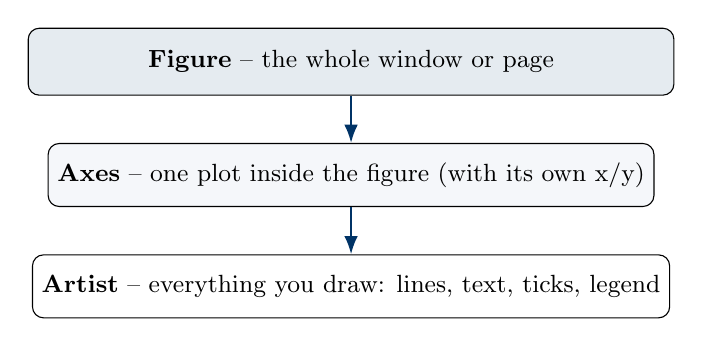
\begin{tikzpicture}[node distance=0.6cm, >=Latex, font=\small]
  \node[draw,rounded corners,fill=PrimaryBlue!10,minimum width=8.2cm,minimum height=0.85cm] (fig) {\textbf{Figure} -- the whole window or page};
  \node[draw,rounded corners,fill=LightGray,minimum width=7.6cm,minimum height=0.8cm,below=of fig] (ax) {\textbf{Axes} -- one plot inside the figure (with its own x/y)};
  \node[draw,rounded corners,fill=white,minimum width=7.0cm,minimum height=0.8cm,below=of ax] (art) {\textbf{Artist} -- everything you draw: lines, text, ticks, legend};
  \draw[->,thick,PrimaryBlue] (fig) -- (ax);
  \draw[->,thick,PrimaryBlue] (ax) -- (art);
\end{tikzpicture}
\end{center}

\vspace{0.1cm}
\begin{tcolorbox}[lecturebox,title=Mental model]
A \keyword{Figure} is the canvas. It holds one or more \keyword{Axes} (each is one chart). Every line, label, and tick on those axes is an \keyword{Artist}. Almost every customization changes some Artist's properties.
\end{tcolorbox}
\end{frame}


\begin{frame}[fragile]
\frametitle{Pyplot vs.\ the Object-Oriented Interface}
\small
Matplotlib offers two styles. They produce identical figures.

\vspace{0.12cm}
\begin{columns}[T,totalwidth=0.98\textwidth]
\begin{column}{0.49\textwidth}
\textbf{Pyplot (quick, MATLAB-like)}
\begin{lstlisting}[style=pycodesmall]
import matplotlib.pyplot as plt

plt.plot([1, 2, 3], [4, 1, 5])
plt.title("Quick plot")
plt.xlabel("x")
plt.ylabel("y")
plt.show()
\end{lstlisting}
\end{column}
\begin{column}{0.49\textwidth}
\textbf{Object-oriented (recommended)}
\begin{lstlisting}[style=pycodesmall]
fig, ax = plt.subplots()

ax.plot([1, 2, 3], [4, 1, 5])
ax.set_title("OO plot")
ax.set_xlabel("x")
ax.set_ylabel("y")
plt.show()
\end{lstlisting}
\end{column}
\end{columns}

\vspace{0.15cm}
\begin{bluebox}{Which to use}
Use \codeword{plt.\dots} for quick exploration. Use \keyword{Figure} and \keyword{Axes} objects (\codeword{fig, ax = plt.subplots()}) for any plot you will customize, save, or reuse. The OO style scales to multi-panel figures cleanly.
\end{bluebox}
\end{frame}


\begin{frame}[fragile]
\frametitle{Basic Charts}
\small
\begin{lstlisting}[style=pycode]
import numpy as np, matplotlib.pyplot as plt
x = np.linspace(0, 10, 50)
y = np.sin(x)

fig, ax = plt.subplots()

ax.plot(x, y, label="sin(x)")        # line plot
ax.scatter(x, y, s=20, c="red")      # scatter
ax.bar(["A", "B", "C"], [3, 7, 5])   # bar chart
ax.hist(np.random.randn(1000), bins=30)   # histogram
ax.pie([30, 45, 25], labels=["A", "B", "C"], autopct="%.0f%%")
\end{lstlisting}

\renewcommand{\arraystretch}{1.20}
\begin{tabularx}{\linewidth}{>{\bfseries}p{2.0cm}X}
\toprule
Chart & Use it for \\
\midrule
line       & ordered or continuous data over an axis (e.g.\ time) \\
scatter    & relationship between two numeric variables \\
bar        & comparing categories \\
histogram  & distribution of one numeric variable \\
pie        & shares of a whole (use \keyword{sparingly}; bars are usually clearer) \\
\bottomrule
\end{tabularx}
\end{frame}


\begin{frame}[fragile]
\frametitle{Customization and Subplots}
\small
\begin{lstlisting}[style=pycode]
fig, axes = plt.subplots(2, 2, figsize=(8, 6))   # 2x2 grid

axes[0, 0].plot(x, np.sin(x), color="navy",
                linestyle="--", linewidth=2, marker="o")
axes[0, 0].set_title("Sine")
axes[0, 0].set(xlabel="x", ylabel="sin(x)")
axes[0, 0].legend(["sin"], loc="upper right")
axes[0, 0].grid(alpha=0.3)
axes[0, 1].scatter(x, np.cos(x), c=x, cmap="viridis")
axes[1, 0].bar(["A", "B"], [10, 20])
axes[1, 1].hist(np.random.randn(500), bins=20)

fig.suptitle("Four-panel figure")
fig.tight_layout()
fig.savefig("plot.png", dpi=300, bbox_inches="tight")
\end{lstlisting}

\begin{tcolorbox}[lecturebox,title=Saving figures]
\codeword{savefig} accepts PNG, SVG, and PDF. Use \codeword{dpi=300} for print, \codeword{bbox\_inches="tight"} to crop whitespace, and SVG/PDF for vector quality in reports and slides.
\end{tcolorbox}
\end{frame}


\begin{frame}[fragile]
\frametitle{Seaborn: Statistical Plotting}
\small
\keyword{Seaborn} sits on top of Matplotlib and produces statistical charts directly from a DataFrame.

\vspace{0.12cm}
\begin{lstlisting}[style=pycode]
import seaborn as sns
import matplotlib.pyplot as plt

sns.set_theme(style="whitegrid")        # clean default look

# Distribution plots
sns.histplot(data=df, x="age", bins=20, kde=True)
sns.kdeplot(data=df,  x="age", hue="dept", fill=True)
sns.ecdfplot(data=df, x="age")

plt.show()
\end{lstlisting}

\begin{bluebox}{Why prefer Seaborn?}
Seaborn understands DataFrames natively. Pass \codeword{data=df}, name your columns by string, and it handles axes, legends, and statistical aesthetics for you. The result is shorter code and better defaults.
\end{bluebox}
\end{frame}


\begin{frame}[fragile]
\frametitle{Categorical and Relational Plots}
\small
\begin{lstlisting}[style=pycode]
# Categorical (one axis is a category)
sns.boxplot(data=df,    x="dept", y="score")
sns.violinplot(data=df, x="dept", y="score", inner="quartile")
sns.stripplot(data=df,  x="dept", y="score", jitter=True)
sns.barplot(data=df,    x="dept", y="score", estimator="mean")
sns.countplot(data=df,  x="dept")

# Relational (both axes are numeric)
sns.scatterplot(data=df, x="age", y="score",
                hue="dept", size="hours", style="gender")
sns.lineplot(data=ts,    x="date", y="price", hue="ticker")
\end{lstlisting}

\begin{tcolorbox}[lecturebox,title=The hue / size / style trio]
Most Seaborn functions accept \codeword{hue}, \codeword{size}, and \codeword{style}. They map a column to color, marker size, or marker shape, letting you encode \keyword{up to five dimensions} on a 2-D chart.
\end{tcolorbox}
\end{frame}


\begin{frame}[fragile]
\frametitle{Heatmaps, Pair Plots, and Styling}
\small
\begin{lstlisting}[style=pycode]
# Correlation heatmap
corr = df.select_dtypes("number").corr()
sns.heatmap(corr, annot=True, cmap="coolwarm",
            vmin=-1, vmax=1, square=True)

# Pair plot: every numeric pair as a scatter, diagonals as histograms
sns.pairplot(df, hue="dept", diag_kind="kde")

# Theming
sns.set_theme(style="whitegrid", palette="deep", font_scale=1.1)
plt.rcParams["figure.dpi"] = 120
\end{lstlisting}

\renewcommand{\arraystretch}{1.20}
\begin{tabularx}{\linewidth}{>{\bfseries}p{3.4cm}X}
\toprule
Function level & Returns \\
\midrule
Axes-level (\codeword{histplot}, \codeword{boxplot}, \codeword{scatterplot}) & a single \keyword{Axes}; you control the figure \\
Figure-level (\codeword{pairplot}, \codeword{relplot}, \codeword{catplot}) & a multi-panel \keyword{Figure} (\codeword{FacetGrid}) \\
\bottomrule
\end{tabularx}
\end{frame}


% ============================================================
% MODULE 5 TITLE SLIDE
% ============================================================
\begin{noheadline}
\begin{frame}
\frametitle{Module 5: EXPLORATORY DATA ANALYSIS (EDA)}
\vspace{1.2cm}
\begin{center}
  {\fontsize{30}{36}\selectfont\textbf{Module 5}}\\[0.35cm]
  {\fontsize{22}{28}\selectfont EXPLORATORY DATA ANALYSIS (EDA)}\\[0.7cm]
  \tcbox[colback=PrimaryBlue!6,colframe=PrimaryBlue,arc=3mm,boxrule=1pt,left=8mm,right=8mm,top=4mm,bottom=4mm,fontupper=\Large]{From raw data to insight: quality, distributions, and patterns}
\end{center}
\end{frame}
\end{noheadline}


% ============================================================
% MODULE 5 CONTENT SLIDE
% ============================================================
\begin{frame}
\frametitle{Module Content}
\small
This module covers a systematic process to understand any dataset --- from quality checks to statistical profiling and machine learning readiness.

\vspace{0.16cm}
\begin{columns}[T,totalwidth=0.96\textwidth]
\begin{column}{0.48\textwidth}
\begin{itemize}\setlength\itemsep{0.08cm}
  \item \keyword{EDA as a process}: the question-explore-visualize-hypothesize loop.
  \item \keyword{Data quality assessment}: missing values, duplicates, and anomalies.
  \item \keyword{Univariate analysis}: distributions, histograms, and summary statistics.
  \item \keyword{Bivariate and multivariate analysis}: correlations and relationships.
\end{itemize}
\end{column}
\begin{column}{0.48\textwidth}
\begin{itemize}\setlength\itemsep{0.08cm}
  \item \keyword{Outlier detection}: IQR, z-scores, and visual methods.
  \item \keyword{ML readiness}: leakage, class imbalance, and feature scaling.
  \item \keyword{Worked example}: a full EDA skeleton on the Titanic dataset.
\end{itemize}
\end{column}
\end{columns}
\end{frame}


% ============================================================
% 5.5 EDA
% ============================================================
\begin{frame}[fragile]
\frametitle{Exploratory Data Analysis as a Process}
\small
\keyword{EDA} is not a single command. It is a structured loop of asking questions and looking at the data until you understand it well enough to model it.

\vspace{0.18cm}
\begin{center}
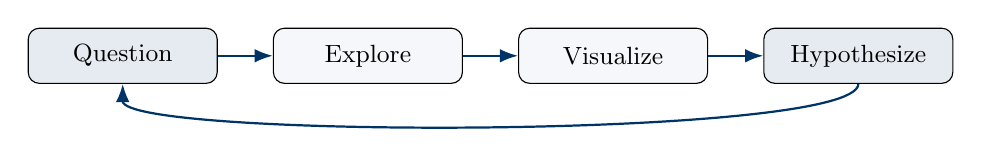
\begin{tikzpicture}[node distance=0.7cm, >=Latex, font=\small]
  \node[draw,rounded corners,fill=PrimaryBlue!10,minimum width=2.4cm,minimum height=0.7cm] (q) {Question};
  \node[draw,rounded corners,fill=LightGray,minimum width=2.4cm,minimum height=0.7cm,right=of q] (e) {Explore};
  \node[draw,rounded corners,fill=LightGray,minimum width=2.4cm,minimum height=0.7cm,right=of e] (v) {Visualize};
  \node[draw,rounded corners,fill=PrimaryBlue!10,minimum width=2.4cm,minimum height=0.7cm,right=of v] (h) {Hypothesize};
  \draw[->,thick,PrimaryBlue] (q) -- (e);
  \draw[->,thick,PrimaryBlue] (e) -- (v);
  \draw[->,thick,PrimaryBlue] (v) -- (h);
  \draw[->,thick,PrimaryBlue] (h.south) .. controls +(0,-0.7) and +(0,-0.7) .. (q.south);
\end{tikzpicture}
\end{center}

\vspace{0.1cm}
\begin{tcolorbox}[lecturebox,title=The deliverable]
Good EDA produces a short report with three sections: \keyword{observations} (what we saw), \keyword{hypotheses} (what we now suspect), and \keyword{recommendations} (what to do next: clean, model, collect more).
\end{tcolorbox}
\end{frame}


\begin{frame}[fragile]
\frametitle{Data Quality Assessment}
\small
Before any analysis, check four properties of the dataset.

\vspace{0.15cm}
\renewcommand{\arraystretch}{1.30}
\begin{tabularx}{\linewidth}{>{\bfseries}p{2.6cm}X}
\toprule
Dimension & What to check \\
\midrule
Completeness  & How many missing values per column? \codeword{df.isna().mean()} as a fraction. \\
Consistency   & Same units, same date format, same spelling for categories (\texttt{"USA"} vs \texttt{"U.S."}). \\
Accuracy      & Plausible ranges (no negative ages, no temperatures of 999). \\
Timeliness    & Is the data fresh enough for the question? \\
\bottomrule
\end{tabularx}

\vspace{0.18cm}
\begin{lstlisting}[style=pycode]
# Quick quality snapshot
df.isna().mean().sort_values(ascending=False)   # % missing per col
df.duplicated().sum()                           # duplicate rows
df["age"].between(0, 120).all()                 # range check
df["country"].value_counts()                    # spot odd categories
\end{lstlisting}
\end{frame}


\begin{frame}[fragile]
\frametitle{Univariate Analysis}
\small
Look at one column at a time. Characterize its \keyword{distribution}: center, spread, and shape.

\vspace{0.12cm}
\begin{lstlisting}[style=pycode]
df["age"].describe()                  # mean, std, quartiles
df["age"].skew()                      # > 0 long right tail
df["age"].kurt()                      # heavier tails than normal

import seaborn as sns
sns.histplot(df["age"], bins=30, kde=True)
sns.boxplot(x=df["age"])              # see outliers and IQR
\end{lstlisting}

\renewcommand{\arraystretch}{1.20}
\begin{tabularx}{\linewidth}{>{\bfseries}p{2.4cm}X}
\toprule
Statistic & Interpretation \\
\midrule
Mean / Median  & center of the distribution; large gap suggests skew or outliers \\
Std / IQR      & spread; IQR is robust to outliers \\
Skewness       & asymmetry: 0 is symmetric, $>$0 right-skewed, $<$0 left-skewed \\
Kurtosis       & tail weight: $>$0 heavier tails, more outliers than a normal \\
\bottomrule
\end{tabularx}
\end{frame}


\begin{frame}[fragile]
\frametitle{Bivariate and Multivariate Analysis}
\small
\begin{lstlisting}[style=pycode]
# Two numeric columns: correlation and scatter
df[["age", "score"]].corr()
sns.scatterplot(data=df, x="age", y="score")

# Numeric vs.\ category: grouped statistics and box plots
df.groupby("dept")["score"].agg(["mean", "std", "count"])
sns.boxplot(data=df, x="dept", y="score")

# Two categories: cross-tabulation
pd.crosstab(df["dept"], df["pass"], normalize="index")

# All numeric columns at once
sns.heatmap(df.corr(numeric_only=True), annot=True, cmap="coolwarm")
sns.pairplot(df, hue="dept")
\end{lstlisting}

\begin{bluebox}{Correlation is not causation}
A strong correlation tells you two columns \keyword{move together}. It does not tell you whether one \emph{causes} the other, or whether a third variable drives both. Always pair correlations with domain reasoning.
\end{bluebox}
\end{frame}


\begin{frame}[fragile]
\frametitle{Outlier Detection}
\small
Outliers are values far from the rest of the data. Detect them with simple statistical rules and confirm visually.

\vspace{0.12cm}
\begin{lstlisting}[style=pycode]
# IQR (interquartile range) method - robust, non-parametric
Q1, Q3 = df["price"].quantile([0.25, 0.75])
IQR = Q3 - Q1
mask = (df["price"] < Q1 - 1.5 * IQR) | (df["price"] > Q3 + 1.5 * IQR)
outliers = df[mask]

# Z-score method - assumes roughly normal distribution
from scipy import stats
z = np.abs(stats.zscore(df["price"]))
outliers = df[z > 3]

# Visual check
sns.boxplot(x=df["price"])
\end{lstlisting}

\begin{tcolorbox}[lecturebox,title=Decide before you delete]
Some outliers are \keyword{errors} (impossible values, typos) and should be removed or corrected. Others are \keyword{rare but real} (a billionaire in a salary dataset) and may be the most informative points. Always investigate before dropping.
\end{tcolorbox}
\end{frame}


\begin{frame}[fragile]
\frametitle{Concerns Specific to Machine Learning}
\small
EDA for ML projects has two extra concerns that easy to miss.

\vspace{0.18cm}
\begin{columns}[T,totalwidth=0.96\textwidth]
\begin{column}{0.5\textwidth}
\textbf{\keyword{Target leakage}}
\begin{itemize}\setlength\itemsep{0.04cm}
  \item A feature that contains future or target-derived information.
  \item Example: predicting churn using \texttt{cancellation\_date}.
  \item Symptom: a single feature is suspiciously predictive.
  \item Fix: remove or rebuild the feature using only data available at prediction time.
\end{itemize}
\end{column}
\begin{column}{0.46\textwidth}
\textbf{\keyword{Class imbalance}}
\begin{itemize}\setlength\itemsep{0.04cm}
  \item One class dominates the target.
  \item Example: 99\% legitimate, 1\% fraud.
  \item Symptom: high accuracy but useless predictions.
  \item Fix: report \keyword{precision/recall/F1}, resample, or use class weights.
\end{itemize}
\end{column}
\end{columns}

\vspace{0.15cm}
\begin{bluebox}{Catch these in EDA}
Both problems are visible in basic EDA. \codeword{value\_counts()} on the target reveals imbalance. A correlation matrix that has one feature near $\pm 1$ with the target screams \emph{leakage}.
\end{bluebox}
\end{frame}


\begin{frame}[fragile]
\frametitle{A Worked EDA Skeleton: Titanic}
\small
A typical first-pass EDA on a tabular dataset.

\vspace{0.12cm}
\begin{lstlisting}[style=pycode]
import pandas as pd, seaborn as sns, matplotlib.pyplot as plt

df = pd.read_csv("titanic.csv")

# 1. SHAPE & TYPES
df.shape, df.dtypes, df.head()

# 2. QUALITY
df.isna().mean().sort_values(ascending=False)
df.duplicated().sum()

# 3. UNIVARIATE
df["Age"].describe()
sns.histplot(df["Age"].dropna(), bins=30, kde=True)
df["Survived"].value_counts(normalize=True)        # class balance

# 4. BIVARIATE / TARGET
df.groupby("Sex")["Survived"].mean()
df.groupby("Pclass")["Survived"].mean()
sns.heatmap(df.corr(numeric_only=True), annot=True)

# 5. OUTPUT a short report:
#    observations -> hypotheses -> next steps
\end{lstlisting}
\end{frame}


% ============================================================
% THANK YOU
% ============================================================
\begin{frame}
\frametitle{Thank You}
\vspace{1.75cm}
\begin{center}
{\fontsize{34}{40}\selectfont \textbf{Thank you!}}\\[0.45cm]
{\fontsize{18}{22}\selectfont Questions and discussion}
\end{center}
\vspace{0.80cm}
\begin{tcolorbox}[lecturebox,title=Course takeaway]
Data science is the discipline of turning raw data into reliable answers. The tools change; the workflow --- inspect, clean, visualize, hypothesize --- does not.
\end{tcolorbox}
\end{frame}


\end{document}
